\renewcommand*{\arraystretch}{1.1}

\subsection*{Interactive / update / 1}
\label{section:interactive-update-01}

% change \emph{} to use sans-serif font
\let\oldemph\emph
\renewcommand{\emph}[1]{{\footnotesize \sf #1}}

\renewcommand{\currentQueryCard}{1}
\marginpar{
	\raggedleft
	\vspace{0.22ex}

	\queryRefCard{interactive-update-01}{IU}{1}\\
	\queryRefCard{interactive-update-02}{IU}{2}\\
	\queryRefCard{interactive-update-03}{IU}{3}\\
	\queryRefCard{interactive-update-04}{IU}{4}\\
	\queryRefCard{interactive-update-05}{IU}{5}\\
	\queryRefCard{interactive-update-06}{IU}{6}\\
	\queryRefCard{interactive-update-07}{IU}{7}\\
	\queryRefCard{interactive-update-08}{IU}{8}\\
}


\noindent\begin{tabularx}{\queryCardWidth}{|>{\queryPropertyCell}p{\queryPropertyCellWidth}|X|}
	\hline
	query & Interactive / update / 1 \\ \hline
%
	title & Add Person \\ \hline
%
	pattern & \multicolumn{1}{c|}{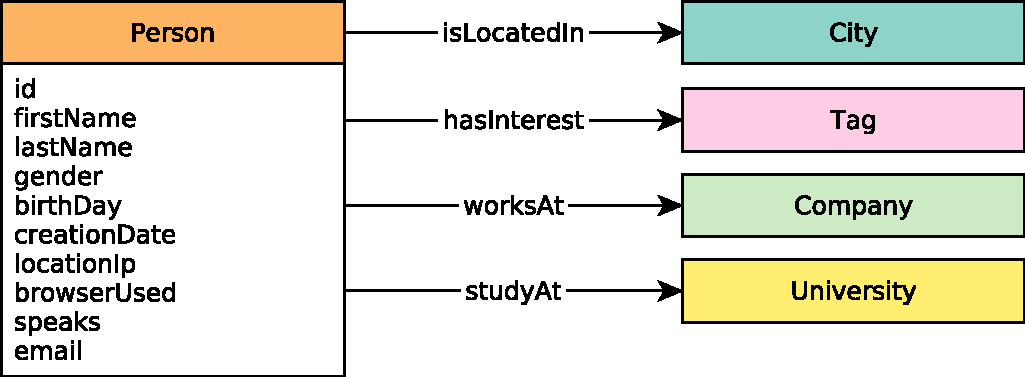
\includegraphics[scale=\patternscale,margin=0cm .2cm]{patterns/interactive-update-01}} \\ \hline
%
	desc. & Add a \emph{Person} \textbf{node}, connected to the network by 4
possible \textbf{edge} types.
 \\ \hline
%
	
		params &
		\innerCardVSpace{\begin{tabularx}{\attributeCardWidth}{|>{\paramNumberCell}c|>{\varNameCell}M|>{\typeCell}m{\typeWidth}|Y|} \hline
		$\mathsf{1}$ & Person.id
 & ID
 &  \\ \hline
		$\mathsf{2}$ & Person.firstName
 & String
 &  \\ \hline
		$\mathsf{3}$ & Person.lastName
 & String
 &  \\ \hline
		$\mathsf{4}$ & Person.gender
 & String
 &  \\ \hline
		$\mathsf{5}$ & Person.birthDay
 & Date
 &  \\ \hline
		$\mathsf{6}$ & Person.creationDate
 & DateTime
 &  \\ \hline
		$\mathsf{7}$ & Person.locationIp
 & String
 &  \\ \hline
		$\mathsf{8}$ & Person.browserUsed
 & String
 &  \\ \hline
		$\mathsf{9}$ & Person-isLocatedIn-\textgreater{}City.id
 & ID
 &  \\ \hline
		$\mathsf{10}$ & Person.speaks
 & \{String\}
 &  \\ \hline
		$\mathsf{11}$ & Person.email
 & \{String\}
 &  \\ \hline
		$\mathsf{12}$ & Person-hasInterest-\textgreater{}Tag.id
 & \{ID\}
 &  \\ \hline
		$\mathsf{13}$ & (Person-studyAt-\textgreater{}University.id,
Person-studyAt-\textgreater{}.classYear)
 & \{(ID, 32-bit Integer)\}
 &  \\ \hline
		$\mathsf{14}$ & (Person-workAt-\textgreater{}Company.id,
Person-workAt-\textgreater{}.workFrom)
 & \{(ID, 32-bit Integer)\}
 &  \\ \hline
		\end{tabularx}}\innerCardVSpace \\ \hline
	
%
	
%
	%
	%
	%
	%
\end{tabularx}
\queryCardVSpace

% change \emph back to the old one
\renewcommand{\emph}[1]{\oldemph{#1}}